\documentclass[10pt]{article}


\usepackage[lmargin=2cm, rmargin=2cm, top=1.5cm, bottom=1.5cm]{geometry}
\usepackage{longtable,multirow,booktabs}
\usepackage{mathrsfs} % para formato de letra
\usepackage[spanish]{babel}
\usepackage[utf8]{inputenc}
\usepackage{amsmath}
\usepackage{amsfonts}
\usepackage{amssymb}
\usepackage{graphicx}
\usepackage{tikz}
\usepackage{float}
\usepackage{dsfont}%Sirve para poner el simbolo de los reales
\graphicspath{imagenes}
\usepackage{hyperref}


\title{\bfseries \huge {PostgreSQL} }
\author{Ezequiel Remus: $<ezequielremus@gmail.com>$}
\date{}

%%%%%%%%%%%%%%%%%%%%%%%%%%%%%%%%%%%%%%%%%%%%%%%%%%%%%%%%%%%%%%%%
%						Ayudas                                 %
%%%%%%%%%%%%%%%%%%%%%%%%%%%%%%%%%%%%%%%%%%%%%%%%%%%%%%%%%%%%%%%%

%\textcolor{LimeGreen}{Hola}
%\colorbox{LimeGreen}{Hola}
%\fcolorbox{LimeGreen}{White}{Hola}
%\fcolorbox{Black}{LimeGreen}{Hola}

%\definecolor{Micolor1}{RGB}{193,124,250}
%\textcolor{Micolor1}{Hola}

%%%%%%%%%%%%%%%%%%%%%%%%%%%%%%%%%%%%%%%%%%%%%%%%%%%%%%%%%%%%%%%%

%%%%%%%%%%%%%%%%%%%%%%%%%%%%%%%%%%%%%%%%%%%%%%%%%%%%%%%%%%%%%%%%
%			 	  Definciciones de Variables                   %
%%%%%%%%%%%%%%%%%%%%%%%%%%%%%%%%%%%%%%%%%%%%%%%%%%%%%%%%%%%%%%%%
%%%%%%%%%%%
% COLORES %
%%%%%%%%%%%
\definecolor{R}{RGB}{176, 11, 11}
\definecolor{B}{RGB}{52, 75, 201}
\definecolor{G}{RGB}{20, 176, 18}
\definecolor{M}{RGB}{133, 71, 33}
\definecolor{Mag}{RGB}{143, 19, 135}

%%%%%%%%%%%
%  TEXTO  %
%%%%%%%%%%%
\newcommand{\py}[1]{{\textcolor{B}{Python} #1}}
\newcommand{\django}[2]{{\textcolor{G}{Django} #2}}
\newcommand{\rest}[1]{{\textcolor{Mag}{REST} #1}}
\newcommand{\djrest}[1]{{\textcolor{Mag}{Django Rest} #1}}
\newcommand{\http}[1]{{\textcolor{B}{HTTP} #1}}
\newcommand{\enlaces}[1]{{\textcolor{G}{URL} #1}}
\newcommand{\postgres}[1]{{\textcolor{R}{PostgreSQL} #1}}
\newcommand{\unix}[1]{{\textcolor{B}{UNIX} #1}}
\newcommand{\mvcc}[1]{{\textcolor{B}{MVCC} #1}}
\newcommand{\psql}[1]{{\textcolor{B}{psql} #1}}
\newcommand{\pgAdmin}[1]{{\textcolor{B}{pgAdmin} #1}}
%%%%%%%%%%%%%%%%%%%%%%%%%%%%%%%%%%%%%%%%%%%%%%%%%%%%%%%%%%%%%%%%
%						Inicio del documento                   %
%%%%%%%%%%%%%%%%%%%%%%%%%%%%%%%%%%%%%%%%%%%%%%%%%%%%%%%%%%%%%%%%

\begin{document}
\renewcommand{\tablename}{Tabla}
%\pagestyle{myheadings}
%TITULO
%modificar el formato del titulo
\maketitle
\newpage

\textbf{Resumen}

Este texto es una traducción del tutorial presentado por \postgres{} el cual se puede encontrar en el siguiente link:

\textbf{El tutorial}
\url{https://www.postgresqltutorial.com}

\tableofcontents
\newpage


\section{Introducción}
\subsection{¿Qué es PostgreSQL?}
\postgres{} es una base de datos relacional de propósito general de codigo abierto. \postgres{} fue desarrollada sobre la base de POSTGRES 4.2 en el departamento de Ciencias de la Computación de la Universidad de Berkeley en California.

\postgres{} fue diseñada para correr sobre plataformas tipo \unix{}. De todos modos, luego de un tiempo se desarrollo para ser portable para que esta pueda emplearce en plataformas \textbf{Mac OS X}, \textbf{Solaris} y \textbf{Windows}. 

Como dijimos \postgres{0} es gratis y de codigo abierto, por lo tanto eres libre de modificar y distribuir de la forma que mas te plazca.

\postgres{} no necesita de un mantenimiento extenso, ya que es bastante estable. Por lo tanto, si desarrollas aplicaciones basadas en \postgres{} el costo total sera minimo.

\subsection{Características}
\begin{itemize}
\item \textit{User-defined types}: Tipos definidos por el usuario
\item \textit{Table inheritance}: Tablas de herencia
\item \textit{Sophisticated locking mechanism}: Un mecanismo de busqueda sofisticado
\item \textit{Foreign key referential integrity}: 
Integridad referencial de clave externa  
\item \textit{Views, rules, subquery}: 
Vistas, reglas, subconsulta
\item \textit{Nested transactions (savepoints)}: Transacciones anidadas (puntos de guardado)
\item \textit{Multi-version concurrency control (\mvcc{}) :} 
Control de concurrencia de versiones múltiples
\item \textit{Asynchronous replication} : Replicación asincrona
\end{itemize}



Las versiones mas recientes de \postgres{} soportan las siguientes caracteristicas:
\\
\begin{itemize}
\item Native Microsoft Windows Server version
\item Table spaces
\item Point-in-time recovery

\end{itemize}

\subsection{¿Porque se destaca \postgres{}?}
\postgres{} es el primer gestor de bases de datos que implementa  un control de concurrencia de versiones multiples (\mvcc{}). 

\postgres{} es un sistema de gestión de bases de datos relacionales de objetos de propósito general. Este te permite agregar funciones personalizadas desarrolladas usando diferentes  lenguajes de programación como C/C++, Java, etc.

\postgres{} fue diseñado para ser extensible. En \postgres{}, tu puedes definir tus propios tipos de datos, inices, lenguajes funcionales, etc. Si no te agreada o sirve alguna parte del sistema, siempre podras desarrrollar un plugin para mejorarlo para satisfacer tus propios requerimientos.

Si necesitas soporte, hay una gran comunidad la cual estara dispuesta a ayudarte. Podras encontrar la respuestas por cualquier problema con los que te cruces mientras trabajas.



\subsection{Instalación}
Todo lo necesario para instalar PostgreSQL esta acá:
\\ \\
\enlaces{} : \url{https://www.postgresql.org/download/}  


\section{Comandos Básicos}
\subsection{Conección a un Servidor de Base de Datos \postgres{}}
Cuando instalas \postgres{} se instalan una serie de herramientas que trabajan directamente con la base de datos. 
Con estas podras conectarte a dicha base de datos via \psql{}
o mediante \pgAdmin{}.

\subsubsection{Conectarse a \postgres{} mediante \psql{}}
\psql{} es una programa de interacción con por terminal.
Este te permite interactuar con el servidor de la base de datos 
como ejecutar sentencias SQL y administrar objetos de base de datos.


Los siguientes pasos nos muestran cómo conectarse al servidor de base de datos \postgres{} a través del programa \psql{}:

\begin{itemize}

\item 
Primero, inicie el programa \psql{} y conéctese al servidor de base de datos \postgres{} utilizando el usuario postgres haciendo clic en el icono \psql{} como se muestra a continuación:

\begin{figure}[H]
  \begin{center}
  	 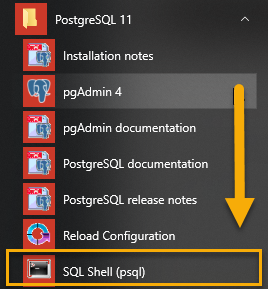
\includegraphics{figures/cap2/img1.png}	 
	 \renewcommand{\arraystretch}{1.3}
	 %\caption{Ciclo Termodinámico Correspondiente al Experimento para El Calculo del $c_k$}
  \end{center}
\end{figure}


\item En segundo lugar, ingrese la información necesaria, como: \textit{Servidor, Base de datos, Puerto, Nombre de usuario y Contraseña}. Presione Entrar para aceptar el valor predeterminado. Sin embargo, debe ingresar la contraseña que configuró durante la instalación.



\begin{figure}[H]
  \begin{center}
  	 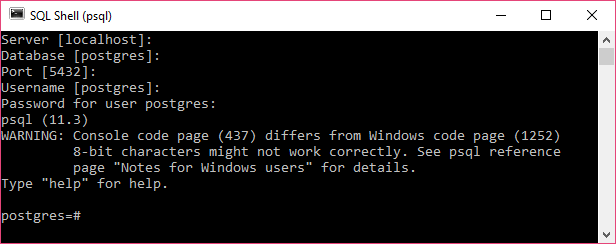
\includegraphics{figures/cap2/img2.png}	 
	 \renewcommand{\arraystretch}{1.3}
	 %\caption{Ciclo Termodinámico Correspondiente al Experimento para El Calculo del $c_k$}
  \end{center}
\end{figure}


\item Tercero, interactúe con el servidor de base de datos PostgreSQL emitiendo una declaración SQL. Puedes probar la siguiente declaración para probarlo:\fbox{\textcolor{B}{SELECT version();}}

\begin{figure}[H]
  \begin{center}
  	 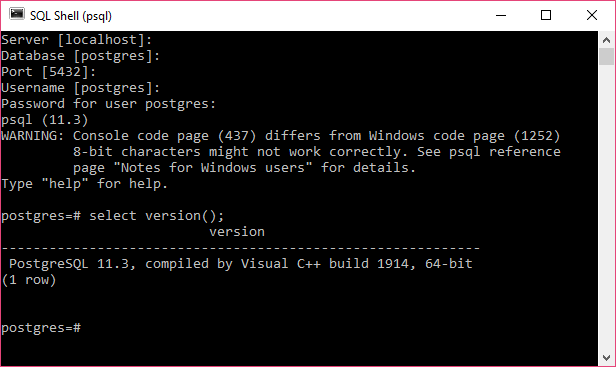
\includegraphics{figures/cap2/img3.png}	 
	 \renewcommand{\arraystretch}{1.3}
	 %\caption{Ciclo Termodinámico Correspondiente al Experimento para El Calculo del $c_k$}
  \end{center}
\end{figure}


No olvides finalizar el comando con punto y coma (;). Después de presionar Enter, psql devolverá la versión actual de PostgreSQL que tiene en el sistema.
\end{itemize}

\subsubsection{Connect to \postgres{} database server using \pgAdmin{}}

La segunda forma de conectarse a una base de datos es mediante la aplicación \pgAdmin{}. Al usar la aplicación \pgAdmin{}, puede interactuar con el servidor de base de datos \postgres{} a través de una interfaz de usuario intuitiva.

A continuación se ilustra cómo conectarse a una base de datos mediante la aplicación \pgAdmin{} GUI:

\begin{itemize}
\item Primero, inicie la aplicación \pgAdmin{}.

\begin{figure}[H]
  \begin{center}
  	 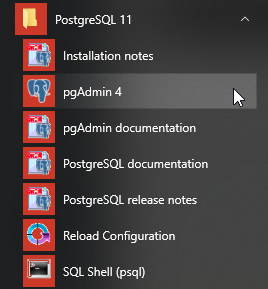
\includegraphics{figures/cap2/img4.png}	 
	 \renewcommand{\arraystretch}{1.3}
	 %\caption{Ciclo Termodinámico Correspondiente al Experimento para El Calculo del $c_k$}
  \end{center}
\end{figure}

La aplicación \pgAdmin{} versión 4 se iniciará en el navegador web como se muestra en la siguiente imagen:

\begin{figure}[H]
  \begin{center}
  	 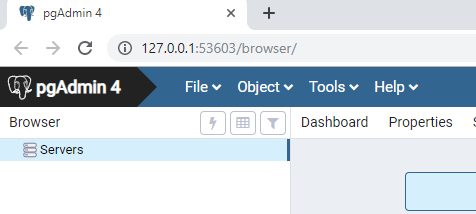
\includegraphics{figures/cap2/img5.png}	 
	 \renewcommand{\arraystretch}{1.3}
	 %\caption{Ciclo Termodinámico Correspondiente al Experimento para El Calculo del $c_k$}
  \end{center}
\end{figure}

\item En segundo lugar, haga clic con el botón derecho en el nodo Servidores y seleccione $Crear> Servidor ...$ para crear un servidor

\begin{figure}[H]
  \begin{center}
  	 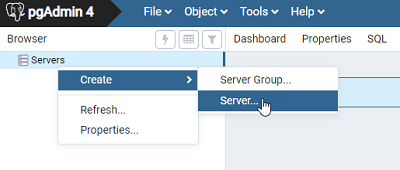
\includegraphics{figures/cap2/img6.png}	 
	 \renewcommand{\arraystretch}{1.3}
	 %\caption{Ciclo Termodinámico Correspondiente al Experimento para El Calculo del $c_k$}
  \end{center}
\end{figure}

\item Tercero, ingrese el nombre del servidor, por ejemplo, \postgres{} y haga clic en la pestaña Conexión

\begin{figure}[H]
  \begin{center}
  	 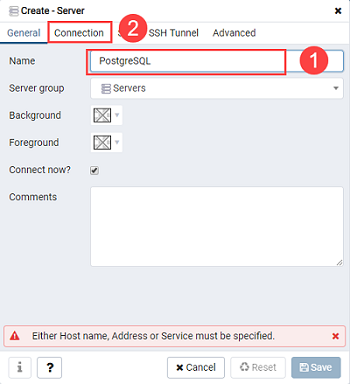
\includegraphics{figures/cap2/img7.png}	 
	 \renewcommand{\arraystretch}{1.3}
	 %\caption{Ciclo Termodinámico Correspondiente al Experimento para El Calculo del $c_k$}
  \end{center}
\end{figure}

\item Cuarto, ingrese el host y la contraseña para el usuario de postgres y haga clic en el botón Guardar:


\begin{figure}[H]
  \begin{center}
  	 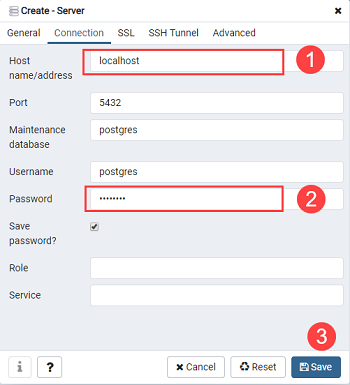
\includegraphics{figures/cap2/img8.png}	 
	 \renewcommand{\arraystretch}{1.3}
	 %\caption{Ciclo Termodinámico Correspondiente al Experimento para El Calculo del $c_k$}
  \end{center}
\end{figure}

\item Quinto, haga clic en el nodo Servidores para expandir el servidor. Por defecto, \postgres{} tiene una base de datos llamada postgres como se muestra a continuación:

\begin{figure}[H]
  \begin{center}
  	 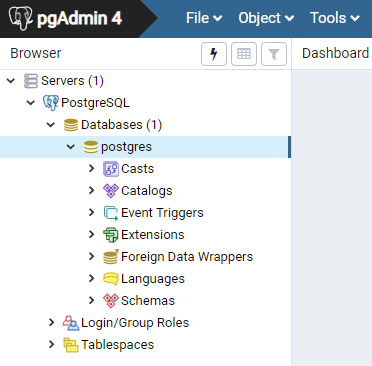
\includegraphics{figures/cap2/img9.png}	 
	 \renewcommand{\arraystretch}{1.3}
	 %\caption{Ciclo Termodinámico Correspondiente al Experimento para El Calculo del $c_k$}
  \end{center}
\end{figure}

\item  Sexto, abra la herramienta de consulta seleccionando el elemento de menú $Herramienta> Herramienta$ de consulta o haga clic en el icono del rayo.

\begin{figure}[H]
  \begin{center}
  	 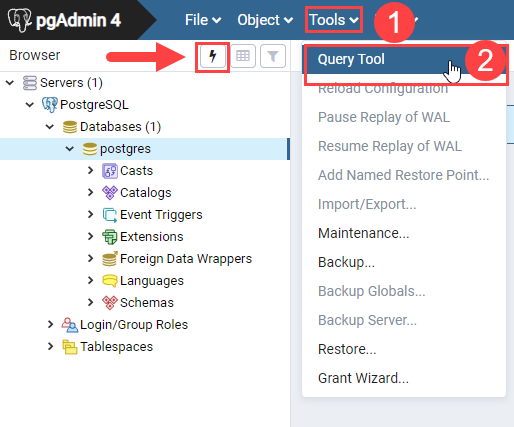
\includegraphics{figures/cap2/img10.png}	 
	 \renewcommand{\arraystretch}{1.3}
	 %\caption{Ciclo Termodinámico Correspondiente al Experimento para El Calculo del $c_k$}
  \end{center}
\end{figure}

\item 
Séptimo, ingrese la consulta en el Editor de consultas, haga clic en el botón Ejecutar, verá el resultado de la consulta en la pestaña Salida de datos:

\begin{figure}[H]
  \begin{center}
  	 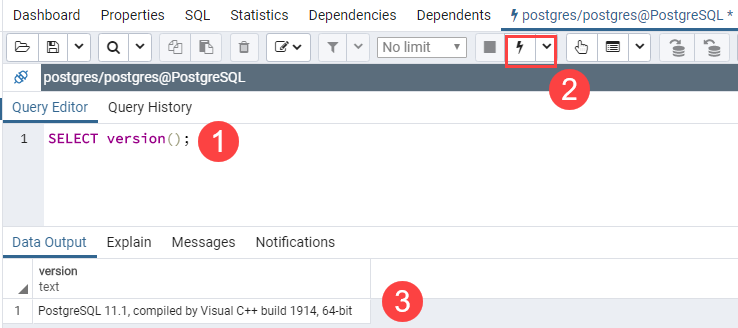
\includegraphics{figures/cap2/img11.png}	 
	 \renewcommand{\arraystretch}{1.3}
	 %\caption{Ciclo Termodinámico Correspondiente al Experimento para El Calculo del $c_k$}
  \end{center}
\end{figure}

\end{itemize}
\subsubsection{Conéctese a la base de datos \postgres{} desde otras aplicaciones}


Cualquier aplicación que admita ODBC o JDBC puede conectarse al servidor de base de datos \postgres{}. Además, si desarrolla una aplicación que utiliza un controlador apropiado, la aplicación también puede conectarse al servidor de base de datos \postgres{}

\begin{itemize}
\item Connect to PostgreSQL from PHP: 

\enlaces{} \url{https://www.postgresqltutorial.com/postgresql-php/connect/}
\item Connect to PostgreSQL from Python:

\enlaces{} \url{https://www.postgresqltutorial.com/postgresql-python/connect/}
\item Connect to PostgreSQL from Java:

\enlaces{} \url{https://www.postgresqltutorial.com/postgresql-jdbc/connecting-to-postgresql-database/}
\end{itemize}

En este tutorial, ha aprendido cómo conectarse al servidor de base de datos \postgres{}  mediante el uso de diferentes herramientas de cliente, incluidas las aplicaciones \psql{} y \pgAdmin{} GUI. Exploremos los objetos de la base de datos \postgres{} y descubramos cómo podemos usarlos en nuestras aplicaciones.







\end{document}